\documentclass{article}\usepackage[]{graphicx}\usepackage[]{xcolor}
% maxwidth is the original width if it is less than linewidth
% otherwise use linewidth (to make sure the graphics do not exceed the margin)
\makeatletter
\def\maxwidth{ %
  \ifdim\Gin@nat@width>\linewidth
    \linewidth
  \else
    \Gin@nat@width
  \fi
}
\makeatother

\definecolor{fgcolor}{rgb}{0.345, 0.345, 0.345}
\newcommand{\hlnum}[1]{\textcolor[rgb]{0.686,0.059,0.569}{#1}}%
\newcommand{\hlstr}[1]{\textcolor[rgb]{0.192,0.494,0.8}{#1}}%
\newcommand{\hlcom}[1]{\textcolor[rgb]{0.678,0.584,0.686}{\textit{#1}}}%
\newcommand{\hlopt}[1]{\textcolor[rgb]{0,0,0}{#1}}%
\newcommand{\hlstd}[1]{\textcolor[rgb]{0.345,0.345,0.345}{#1}}%
\newcommand{\hlkwa}[1]{\textcolor[rgb]{0.161,0.373,0.58}{\textbf{#1}}}%
\newcommand{\hlkwb}[1]{\textcolor[rgb]{0.69,0.353,0.396}{#1}}%
\newcommand{\hlkwc}[1]{\textcolor[rgb]{0.333,0.667,0.333}{#1}}%
\newcommand{\hlkwd}[1]{\textcolor[rgb]{0.737,0.353,0.396}{\textbf{#1}}}%
\let\hlipl\hlkwb

\usepackage{framed}
\makeatletter
\newenvironment{kframe}{%
 \def\at@end@of@kframe{}%
 \ifinner\ifhmode%
  \def\at@end@of@kframe{\end{minipage}}%
  \begin{minipage}{\columnwidth}%
 \fi\fi%
 \def\FrameCommand##1{\hskip\@totalleftmargin \hskip-\fboxsep
 \colorbox{shadecolor}{##1}\hskip-\fboxsep
     % There is no \\@totalrightmargin, so:
     \hskip-\linewidth \hskip-\@totalleftmargin \hskip\columnwidth}%
 \MakeFramed {\advance\hsize-\width
   \@totalleftmargin\z@ \linewidth\hsize
   \@setminipage}}%
 {\par\unskip\endMakeFramed%
 \at@end@of@kframe}
\makeatother

\definecolor{shadecolor}{rgb}{.97, .97, .97}
\definecolor{messagecolor}{rgb}{0, 0, 0}
\definecolor{warningcolor}{rgb}{1, 0, 1}
\definecolor{errorcolor}{rgb}{1, 0, 0}
\newenvironment{knitrout}{}{} % an empty environment to be redefined in TeX

\usepackage{alltt}
\title{\textbf{R Homework Two}}
\author{\textbf{Katherine Wolf}\\ Introduction to Causal Inference (PH252D)\\ \today}
\date{}

% list of latex packages you'll need
\usepackage{float}  % for tables
\usepackage{mathtools}  % for mathematical symbols
\usepackage{bm}  % to bold mathematical symbols like betas
\usepackage{scrextend}  % to indent subsections
\usepackage{xltxtra}
\usepackage{fontspec}
\usepackage{xunicode}
\usepackage[skip=0.5\baselineskip]{caption}  % control caption printing space
\usepackage{longtable}
\usepackage{amsmath}
\usepackage{amsfonts}
\usepackage{bm}
\usepackage{caption}
\usepackage[shortlabels]{enumitem}
\usepackage{txfonts}
\usepackage{dejavu}
\usepackage{mathpazo}

% set fonts
\setmainfont{Palatino Linotype}
\setsansfont{Corbel}
\setmonofont{Consolas}

% make special code formatting
\NewDocumentCommand{\codeword}{v}{%
  \texttt{{#1}}%
}

% set the margins of the document
\usepackage[top=1in, bottom=1in, left=.5in, right=.5in]{geometry}

% remove automatic indenting
\setlength{\parindent}{0pt}



% end the preamble and begin the document
\IfFileExists{upquote.sty}{\usepackage{upquote}}{}
\begin{document}

\maketitle

\section{Time to prevent child malnutrition in Sahel}

\section{A specific data generating process}

  \subsection{Evaluate the positivity assumption in closed form for this data generating process.}
  
For the positivity assumption to hold, there must be a positive (but less than one) probability of receiving the intervention package ($A = 1$) and the standard of care ($A = 0$) within all possible strata of health care access ($W1$) and conflict history ($W2$), i.e., all of the following must hold:

\begin{align*}
0<\mathbb{P}_0(A=1|W1=1,W2=1)<1 \\
0<\mathbb{P}_0(A=1|W1=1,W2=0)<1 \\
0<\mathbb{P}_0(A=1|W1=0,W2=1)<1 \\
0<\mathbb{P}_0(A=1|W1=0,W2=0)<1
\end{align*}

This data generating process specifies
\begin{itemize}
\item That the exogenous factors influencing the value of A are generated as $U_A \sim Uniform(0,1)$, and 
\item That given the exogenous factors $U_A$, the value of $A$ is derministically generated as 
\begin{align*}
A=\mathbb{I}[U_A<logit^{-1}(-0.5+W1-1.5*W2)],
\end{align*}

where $A=1$ if the value of $U_A$ is less than the expression on the right of the inequality sign and $A=0$ otherwise.
\end{itemize}

Since the $logit^{-1}$ function is bounded between 0 and 1, and since $U_A \sim Uniform(0,1)$, i.e., equally likely to be any number from 0 to 1, the probability that $A=1$ conditional on the covariates $W1$ and $W2$ in this data generating system is then the value of $logit^{-1}(-0.5+W1-1.5*W2)$, i.e., 
\begin{align*}
\mathbb{P}_0(A=1|W1,W2)=logit^{-1}(-0.5+W1-1.5*W2).
\end{align*}

To evaluate the positivity assumption in closed form for this data-generating process, then, we can plug the four possible combinations of $W1$ and $W2$ into the equation above. The positivity assumption is satisfied if the equation generates a number between 0 and 1 exclusive for all four possible covariate combinations.

\begin{itemize}
  
  \item For $W1=1, W2=1$:
\begin{align*}
\mathbb{P}_0(A=1|W1=1,W2=1) &= logit^{-1}(-0.5+1-1.5*1) = 0.2689414
\end{align*}

  \item For $W1=1, W2=0$:
\begin{align*}
\mathbb{P}_0(A=1|W1=1,W2=0) &= logit^{-1}(-0.5+1-1.5*0) = 0.6224593
\end{align*}

  \item For $W1=0, W2=1$:
\begin{align*}
\mathbb{P}_0(A=1|W1=0,W2=1) &= logit^{-1}(-0.5+0-1.5*1) = 0.1192029
\end{align*}

  \item For $W1=0, W2=0$:
\begin{align*}
\mathbb{P}_0(A=1|W1=0,W2=0) &= logit^{-1}(-0.5+0-1.5*0) = 0.3775407
\end{align*}
  
\end{itemize}

Since $0 < \mathbb{P}_0(A=1|W1,W2) < 1$ for all four possible combinations of $W1$ and $W2$, the positivity assumption is satisfied.


\newpage
  
\subsection{\textit{Bonus (optional)}: Evaluate the statistical estimand $\Psi(\mathbb{P}_0)$ in closed form for this data generating process.}

The target causal parameter $\Psi^F(\mathbb{P}_{U,X})$ is the difference between the counterfactual probability of survival (of $Y=1$) if all children receive the combination prevention package and the counterfactual probability of survival if all children do not receive the package. (Because $Y$ is a Bernoulli variable, its probabilty of equaling one, $\mathbb{P}(Y=1)$, equals its expectation $\mathbb{E}(Y)$.) Formally,
\begin{align*}
\Psi^F(\mathbb{P}_{U,X})=\mathbb{P}_{U,X}(Y_1=1)-\mathbb{P}_{U,X}(Y_0=1)=\mathbb{E}_{U,X}(Y_1)-\mathbb{E}_{U,X}(Y_0)
\end{align*}

Under the assumptions of the working structural causal model $\mathcal{M}^{\mathcal{F}^*}$, the target causal parameter $\Psi^{F^*}(\mathbb{P}_{U,X})=\mathbb{E}_{U,X}(Y_1)-\mathbb{E}_{U,X}(Y_0)$ is identified by statistical estimand $\Psi(\mathbb{P}_0)$ using the G-computation formula:
\begin{align}
\begin{split}
\Psi(\mathbb{P}_0) &= \mathbb{E}_0[\mathbb{E}_0(Y|A=1,W1,W2)-\mathbb{E}_0(Y|A=0,W1,W2)] \\
&= \sum_{w1,w2}[\mathbb{E}_0(Y|A=1,W1=w1,W2=w2)-\mathbb{E}_0(Y|A=0,W1=w1,W2=w2)]\mathbb{P}_0(W1=w1,W2=w2)
\end{split}
\end{align}

This specific data generating process specifies 
\begin{itemize}

\item That the exogenous factors influencing the value of Y are generated as $U_Y \sim Uniform(0,1)$ and 

\item That, given the exogenous factors $U_Y$, the exposure $A$, and the covariates $W1$ and $W2$, the value of $Y$ is derministically generated as 
\begin{align*}
Y=\mathbb{I}[U_Y<logit^{-1}(-0.75+W1-2W2+2.5*A+A*W1)],
\end{align*}

where $Y=1$ if the value of $U_Y$ is less than the expression on the right of the inequality sign and $Y=0$ otherwise.  

\end{itemize}

Since the $logit^{-1}$ function is bounded between 0 and 1, and since $U_Y \sim Uniform(0,1)$, i.e., equally likely to be any number from 0 to 1, the probability that $Y=1$ conditional on the exposure $A$ and covariates $W1$ and $W2$ in this data generating process is then the value of $logit^{-1}(-0.75+W1-2W2+2.5A+A*W1)$, i.e., 
\begin{align*}
\mathbb{P}_0(Y=1|A,W1,W2)=logit^{-1}(-0.75+W1-2W2+2.5A+A*W1).
\end{align*}
  
Since $Y$ is a Bernoulli random variable, its (conditional) probability of equaling one $\mathbb{P}_0(Y=1|A,W1,W2)$ equals its expectation $\mathbb{E}_0(Y|A,W1,W2)$, i.e.,
\begin{align*}
\mathbb{E}_0(Y|A,W1,W2)=\mathbb{P}_0(Y=1|A,W1,W2)=logit^{-1}(-0.75+W1-2W2+2.5A+A*W1)
\end{align*}

Similarly, for W1 and W2, this specific data generating process specifies 
\begin{itemize}

\item That the exogenous factors influencing the value of W1 and W2 are generated as $U_{W1} \sim Uniform(0,1)$ and $U_{W2} \sim Uniform(0,1)$, respectively, and

\item That, given the exogenous factors $U_{W1}$ and $U_{W2}$, respectively, the values of $W1$ and $W2$ are deterministically generated respectively as 
\begin{align*}
W1=\mathbb{I}[U_{W1}<0.50] \\
W2=\mathbb{I}[U_{W2}<0.50]
\end{align*}

where $W1=1$ or $W2=1$ if the value of $U_W1$ or $U_W2$, respectively, is less than 0.50 and 0 otherwise.  

\end{itemize}

Since $U_{W1}$ and $U_{W2}$ are distributed as $Uniform(0,1)$ and thus equally likely to be any number from 0 to 1, the probability that $W1=1$ and the probability that $W2=1$ are each 0.50, i.e., 

\begin{align*}
P_0(W1=1)=P_0(W2=1)=0.50.
\end{align*}

Since 0 is the only other possible value for each of $W1$ and $W2$, and the total probability must sum to 1, the probability that $W1=0$ and the probability that $W2=0$ are also each 0.50:

\begin{align*}
P_0(W1=0)=1-P_0(W1=1)=1-0.50=0.50 \\
P_0(W2=0)=1-P_0(W2=1)=1-0.50=0.50
\end{align*}

Moreover, since $W1$ and $W2$ are independent in the working structural causal model and this particular data generating process, we can obtain their joint distribution $P_0(W1=w1,W2=w2)$ via multiplication:

\begin{align*}
P_0(W1=w1,W2=w2)=P_0(W1=w1)*P_0(W2=w2)
\end{align*}

Moreover, since $P_0(W1=w1)=P_0(W2=w2)=0.50$ for every possible value of $w1$ and $w2$, $P_0(W1=w1,W2=w2)=P_0(W1=w1)*P_0(W2=w2)=0.5*0.5=0.25$ for every one of the four possible combinations of $w1$ and $w2$.

\vspace{2mm}

Thus to calculate the statistical estimand $\Psi(\mathbb{P}_0)$, we can plug the expressions for the above expected values of $Y$, 

$\mathbb{E}_0(Y|A,W1,W2)$, and the joint probability of $W1=w1$ and $W2=w2$, $P_0(W1=w1,W2=w2)$, into the G-computation formula outlined above in numbered equation (1):



{\scriptsize
\begin{align*}
\Psi(\mathbb{P}_0) &= \sum_{w1,w2}[\mathbb{E}_0(Y|A=1,W1=w1,W2=w2)-\mathbb{E}_0(Y|A=0,W1=w1,W2=w2)]\mathbb{P}_0(W1=w1,W2=w2) \\
&= \sum_{w1,w2}([logit^{-1}(-0.75+W1-2W2+2.5(A=1)+(A=1)W1)-logit^{-1}(-0.75+W1-2W2+2.5(A=0)+(A=0)W1)]*0.25 \\
&= [logit^{-1}(-0.75+1-2*1+2.5*1+1*1) - logit^{-1}(-0.75+1-2*1+2.5*0+0*1)]*0.25 \\
&\qquad + [logit^{-1}(-0.75+1-2*0+2.5*1+1*1) - logit^{-1}(-0.75+1-2*0+2.5*0+0*1)]*0.25 \\
&\qquad + [logit^{-1}(-0.75+0-2*1+2.5*1+1*0) - logit^{-1}(-0.75+0-2*1+2.5*0+0*0)]*0.25 \\
&\qquad + [logit^{-1}(-0.75+0-2*0+2.5*1+1*0) - logit^{-1}(-0.75+0-2*0+2.5*0+0*0)]*0.25 \\
&= 0.506905
\end{align*}\par}

This says that the strata-specific (i.e., (health-care-access-and-conflict-history-specific) conditional probability of survival for those who receive the combination prevention package, averaged with respect to the distribution of the baseline covariates (health care access and confict history), is 0.5069 higher than that of those who do not receive the combination prevention package. Since this data generating process satisfies the positivity assumption and under this data generating process the set of covariates $(W1, W2)$ satisfies the backdoor criterion, for this data generating process, $\Psi(\mathbb{P}_0)$ identifies the average treatment effect $\Psi^F(\mathbb{P}_{U,X})$, the difference between the counterfactual probability of survival if all children receive the combination prevention package and the counterfactual probabiilty of survival if all children do not receive the package.




\newpage

\section{Translate this data generating process into simulations}

\begin{knitrout}
\definecolor{shadecolor}{rgb}{0.969, 0.969, 0.969}\color{fgcolor}\begin{kframe}
\begin{alltt}
\hlkwd{library}\hlstd{(tidyverse)}
\end{alltt}
\end{kframe}
\end{knitrout}


  \subsection{First set the seed to 252.}
  
\begin{knitrout}
\definecolor{shadecolor}{rgb}{0.969, 0.969, 0.969}\color{fgcolor}\begin{kframe}
\begin{alltt}
\hlkwd{set.seed}\hlstd{(}\hlnum{252}\hlstd{)}
\end{alltt}
\end{kframe}
\end{knitrout}
  
  \subsection{Set the number of draws $n = 100,000$.}
  
\begin{knitrout}
\definecolor{shadecolor}{rgb}{0.969, 0.969, 0.969}\color{fgcolor}\begin{kframe}
\begin{alltt}
\hlstd{n} \hlkwb{=} \hlnum{100000}
\end{alltt}
\end{kframe}
\end{knitrout}
  
  \subsection{Sample $n$ independent and identically distributed (i.i.d.) observations of random variable $O=(W1,W2,A,Y) \sim \mathbb{P}_0$.}
  
\begin{knitrout}
\definecolor{shadecolor}{rgb}{0.969, 0.969, 0.969}\color{fgcolor}\begin{kframe}
\begin{alltt}
\hlstd{U_W1} \hlkwb{<-} \hlkwd{runif}\hlstd{(n,} \hlkwc{min}\hlstd{=}\hlnum{0}\hlstd{,} \hlkwc{max}\hlstd{=}\hlnum{1}\hlstd{)}
\hlstd{U_W2} \hlkwb{<-} \hlkwd{runif}\hlstd{(n,} \hlkwc{min}\hlstd{=}\hlnum{0}\hlstd{,} \hlkwc{max}\hlstd{=}\hlnum{1}\hlstd{)}
\hlstd{U_A} \hlkwb{<-} \hlkwd{runif}\hlstd{(n,} \hlkwc{min}\hlstd{=}\hlnum{0}\hlstd{,} \hlkwc{max}\hlstd{=}\hlnum{1}\hlstd{)}
\hlstd{U_Y} \hlkwb{<-} \hlkwd{runif}\hlstd{(n,} \hlkwc{min}\hlstd{=}\hlnum{0}\hlstd{,} \hlkwc{max}\hlstd{=}\hlnum{1}\hlstd{)}

\hlstd{W1} \hlkwb{<-} \hlkwd{as.numeric}\hlstd{(U_W1} \hlopt{<} \hlnum{0.5}\hlstd{)}
\hlstd{W2} \hlkwb{<-} \hlkwd{as.numeric}\hlstd{(U_W2} \hlopt{<} \hlnum{0.5}\hlstd{)}
\hlstd{A} \hlkwb{<-} \hlkwd{as.numeric}\hlstd{(U_A} \hlopt{<} \hlkwd{plogis}\hlstd{(}\hlopt{-}\hlnum{0.5}\hlopt{+}\hlstd{W1}\hlopt{-}\hlnum{1.5}\hlopt{*}\hlstd{W2))}
\hlstd{Y} \hlkwb{<-} \hlkwd{as.numeric}\hlstd{(U_Y} \hlopt{<} \hlkwd{plogis}\hlstd{(}\hlopt{-}\hlnum{0.75}\hlopt{+}\hlstd{W1}\hlopt{-}\hlnum{2}\hlopt{*}\hlstd{W2}\hlopt{+}\hlnum{2.5}\hlopt{*}\hlstd{A}\hlopt{+}\hlstd{A}\hlopt{*}\hlstd{W1))}

\hlstd{X} \hlkwb{<-} \hlkwd{tibble}\hlstd{(W1, W2, A, Y)}
\end{alltt}
\end{kframe}
\end{knitrout}
  
  
  \subsection{\textit{Bonus}: Intervene to set the exposure to the combination package $(A=1)$ and generate the counterfactual outcome $Y_1$. Intervene to set the exposure to the standard of care $(A=0)$ and generate the counterfactual outcomes $Y_0$. Evaluate the causal parameter $\Psi^F(\mathbb{P}_{U,X})$.}
  
\begin{knitrout}
\definecolor{shadecolor}{rgb}{0.969, 0.969, 0.969}\color{fgcolor}\begin{kframe}
\begin{alltt}
\hlstd{Y_1} \hlkwb{<-} \hlkwd{as.numeric}\hlstd{(U_Y} \hlopt{<} \hlkwd{plogis}\hlstd{(}\hlopt{-}\hlnum{0.75}\hlopt{+}\hlstd{W1}\hlopt{-}\hlnum{2}\hlopt{*}\hlstd{W2}\hlopt{+}\hlnum{2.5}\hlopt{*}\hlnum{1}\hlopt{+}\hlnum{1}\hlopt{*}\hlstd{W1))}

\hlstd{Y_0} \hlkwb{<-} \hlkwd{as.numeric}\hlstd{(U_Y} \hlopt{<} \hlkwd{plogis}\hlstd{(}\hlopt{-}\hlnum{0.75}\hlopt{+}\hlstd{W1}\hlopt{-}\hlnum{2}\hlopt{*}\hlstd{W2}\hlopt{+}\hlnum{2.5}\hlopt{*}\hlnum{0}\hlopt{+}\hlnum{0}\hlopt{*}\hlstd{W1))}

\hlstd{Psi_F} \hlkwb{<-} \hlkwd{mean}\hlstd{(Y_1)} \hlopt{-} \hlkwd{mean}\hlstd{(Y_0)}

\hlstd{Psi_F}
\end{alltt}
\begin{verbatim}
## [1] 0.50707
\end{verbatim}
\end{kframe}
\end{knitrout}
 
The above result of $\Psi^F(\mathbb{P}_{U,X}) = 0.5071$ shows that under this data generating process and given the distribution of baseline covariates $W1$ and $W2$ in this population, the difference between the counterfactual probability of survival if all children receive the combination prevention package and the counterfactual probabiilty of survival if all children do not receive the package, i.e., the average treatment effect, is 0.5071.
  
  \subsection{Evaluate the positivity assumption.}
  
For the positivity assumption to hold, there must be a positive (but less than one) probability of receiving the intervention package ($A = 1$) and the standard of care ($A = 0$) within all possible strata of health care access ($W1$) and conflict history ($W2$), i.e., all of the following must hold:

\begin{align*}
0<\mathbb{P}_0(A=1|W1=1,W2=1)<1 \\
0<\mathbb{P}_0(A=1|W1=1,W2=0)<1 \\
0<\mathbb{P}_0(A=1|W1=0,W2=1)<1 \\
0<\mathbb{P}_0(A=1|W1=0,W2=0)<1
\end{align*}

Using this simulated data, we can check the positivity assumption by checking whether the mean of $A$ within each possible stratum of $(W1, W2)$ in the simulated data is between 0 and 1 exclusive:
  
\begin{knitrout}
\definecolor{shadecolor}{rgb}{0.969, 0.969, 0.969}\color{fgcolor}\begin{kframe}
\begin{alltt}
\hlstd{mean_A_W1_1_W2_1} \hlkwb{<-} \hlkwd{mean}\hlstd{(A[W1} \hlopt{==} \hlnum{1} \hlopt{&} \hlstd{W2} \hlopt{==} \hlnum{1}\hlstd{])}
\hlstd{mean_A_W1_1_W2_1}
\end{alltt}
\begin{verbatim}
## [1] 0.271355
\end{verbatim}
\begin{alltt}
\hlstd{mean_A_W1_1_W2_0} \hlkwb{<-} \hlkwd{mean}\hlstd{(A[W1} \hlopt{==} \hlnum{1} \hlopt{&} \hlstd{W2} \hlopt{==} \hlnum{0}\hlstd{])}
\hlstd{mean_A_W1_1_W2_0}
\end{alltt}
\begin{verbatim}
## [1] 0.6221695
\end{verbatim}
\begin{alltt}
\hlstd{mean_A_W1_0_W2_1} \hlkwb{<-} \hlkwd{mean}\hlstd{(A[W1} \hlopt{==} \hlnum{0} \hlopt{&} \hlstd{W2} \hlopt{==} \hlnum{1}\hlstd{])}
\hlstd{mean_A_W1_0_W2_1}
\end{alltt}
\begin{verbatim}
## [1] 0.1190666
\end{verbatim}
\begin{alltt}
\hlstd{mean_A_W1_0_W2_0} \hlkwb{<-} \hlkwd{mean}\hlstd{(A[W1} \hlopt{==} \hlnum{0} \hlopt{&} \hlstd{W2} \hlopt{==} \hlnum{0}\hlstd{])}
\hlstd{mean_A_W1_0_W2_0}
\end{alltt}
\begin{verbatim}
## [1] 0.3756981
\end{verbatim}
\end{kframe}
\end{knitrout}


Thus we have 

\begin{itemize}
  \item For $W1=1,W2=1$:
  \begin{itemize}
    \item $\mathbb{P}_0(A=1|W1=1,W2=1)=0.2714$
    \item $\mathbb{P}_0(A=0|W1=1,W2=1)=1-\mathbb{P}_0(A=1|W1=1,W2=1)=0.7286$
  \end{itemize}
  \item For $W1=1,W2=0$:
  \begin{itemize}
    \item $\mathbb{P}_0(A=1|W1=1,W2=0)=0.6222$
    \item $\mathbb{P}_0(A=0|W1=1,W2=0)=1-\mathbb{P}_0(A=1|W1=1,W2=0)=0.3778$  
  \end{itemize}
  \item For $W1=0,W2=1$:
  \begin{itemize}
    \item $\mathbb{P}_0(A=1|W1=0,W2=1)=0.1191$
    \item $\mathbb{P}_0(A=0|W1=0,W2=1)=1-\mathbb{P}_0(A=1|W1=0,W2=1)=0.8809$  
  \end{itemize}
  \item For $W1=0,W2=0$:
  \begin{itemize}
    \item $\mathbb{P}_0(A=1|W1=0,W2=0)=0.3757$
    \item $\mathbb{P}_0(A=0|W1=0,W2=0)=1-\mathbb{P}_0(A=1|W1=0,W2=0)=0.6243$
  \end{itemize}
\end{itemize}

Since the simulated mean probability of $A=0$ and the simulated mean probability of $A=1$ is between 0 and 1 exclusive for all strata (possible combinations of values of $W1$ and $W2$), the positivity assumption is met.

  \subsection{Evaluate the statistical estimand $\Psi(\mathbb{P}_0)$ and assign the value $\psi_0$ to \texttt{Psi.P0}.}

\begin{knitrout}
\definecolor{shadecolor}{rgb}{0.969, 0.969, 0.969}\color{fgcolor}\begin{kframe}
\begin{alltt}
\hlstd{mean_Y_A_1_W1_1_W2_1} \hlkwb{<-} \hlkwd{mean}\hlstd{(Y[A} \hlopt{==} \hlnum{1} \hlopt{&} \hlstd{W1} \hlopt{==} \hlnum{1} \hlopt{&} \hlstd{W2} \hlopt{==} \hlnum{1}\hlstd{])}

\hlstd{mean_Y_A_0_W1_1_W2_1} \hlkwb{<-} \hlkwd{mean}\hlstd{(Y[A} \hlopt{==} \hlnum{0} \hlopt{&} \hlstd{W1} \hlopt{==} \hlnum{1} \hlopt{&} \hlstd{W2} \hlopt{==} \hlnum{1}\hlstd{])}

\hlstd{P_W1_1_W2_1} \hlkwb{<-} \hlkwd{length}\hlstd{(Y[W1} \hlopt{==} \hlnum{1} \hlopt{&} \hlstd{W2} \hlopt{==} \hlnum{1}\hlstd{])}\hlopt{/}\hlstd{n}


\hlstd{mean_Y_A_1_W1_1_W2_0} \hlkwb{<-} \hlkwd{mean}\hlstd{(Y[A} \hlopt{==} \hlnum{1} \hlopt{&} \hlstd{W1} \hlopt{==} \hlnum{1} \hlopt{&} \hlstd{W2} \hlopt{==} \hlnum{0}\hlstd{])}

\hlstd{mean_Y_A_0_W1_1_W2_0} \hlkwb{<-} \hlkwd{mean}\hlstd{(Y[A} \hlopt{==} \hlnum{0} \hlopt{&} \hlstd{W1} \hlopt{==} \hlnum{1} \hlopt{&} \hlstd{W2} \hlopt{==} \hlnum{0}\hlstd{])}

\hlstd{P_W1_1_W2_0} \hlkwb{<-} \hlkwd{length}\hlstd{(Y[W1} \hlopt{==} \hlnum{1} \hlopt{&} \hlstd{W2} \hlopt{==} \hlnum{0}\hlstd{])}\hlopt{/}\hlstd{n}


\hlstd{mean_Y_A_1_W1_0_W2_1} \hlkwb{<-} \hlkwd{mean}\hlstd{(Y[A} \hlopt{==} \hlnum{1} \hlopt{&} \hlstd{W1} \hlopt{==} \hlnum{0} \hlopt{&} \hlstd{W2} \hlopt{==} \hlnum{1}\hlstd{])}

\hlstd{mean_Y_A_0_W1_0_W2_1} \hlkwb{<-} \hlkwd{mean}\hlstd{(Y[A} \hlopt{==} \hlnum{0} \hlopt{&} \hlstd{W1} \hlopt{==} \hlnum{0} \hlopt{&} \hlstd{W2} \hlopt{==} \hlnum{1}\hlstd{])}

\hlstd{P_W1_0_W2_1} \hlkwb{<-} \hlkwd{length}\hlstd{(Y[W1} \hlopt{==} \hlnum{0} \hlopt{&} \hlstd{W2} \hlopt{==} \hlnum{1}\hlstd{])}\hlopt{/}\hlstd{n}


\hlstd{mean_Y_A_1_W1_0_W2_0} \hlkwb{<-} \hlkwd{mean}\hlstd{(Y[A} \hlopt{==} \hlnum{1} \hlopt{&} \hlstd{W1} \hlopt{==} \hlnum{0} \hlopt{&} \hlstd{W2} \hlopt{==} \hlnum{0}\hlstd{])}

\hlstd{mean_Y_A_0_W1_0_W2_0} \hlkwb{<-} \hlkwd{mean}\hlstd{(Y[A} \hlopt{==} \hlnum{0} \hlopt{&} \hlstd{W1} \hlopt{==} \hlnum{0} \hlopt{&} \hlstd{W2} \hlopt{==} \hlnum{0}\hlstd{])}

\hlstd{P_W1_0_W2_0} \hlkwb{<-} \hlkwd{length}\hlstd{(Y[W1} \hlopt{==} \hlnum{0} \hlopt{&} \hlstd{W2} \hlopt{==} \hlnum{0}\hlstd{])}\hlopt{/}\hlstd{n}


\hlcom{# underscore instead of period because periods are of the devil}

\hlstd{Psi_P0} \hlkwb{<-}
  \hlstd{(mean_Y_A_1_W1_1_W2_1} \hlopt{-} \hlstd{mean_Y_A_0_W1_1_W2_1)}\hlopt{*}\hlstd{P_W1_1_W2_1} \hlopt{+}
  \hlstd{(mean_Y_A_1_W1_1_W2_0} \hlopt{-} \hlstd{mean_Y_A_0_W1_1_W2_0)}\hlopt{*}\hlstd{P_W1_1_W2_0} \hlopt{+}
  \hlstd{(mean_Y_A_1_W1_0_W2_1} \hlopt{-} \hlstd{mean_Y_A_0_W1_0_W2_1)}\hlopt{*}\hlstd{P_W1_0_W2_1} \hlopt{+}
  \hlstd{(mean_Y_A_1_W1_0_W2_0} \hlopt{-} \hlstd{mean_Y_A_0_W1_0_W2_0)}\hlopt{*}\hlstd{P_W1_0_W2_0}

\hlstd{Psi_P0}
\end{alltt}
\begin{verbatim}
## [1] 0.5041414
\end{verbatim}
\end{kframe}
\end{knitrout}
  
  \subsection{Interpret $\Psi(\mathbb{P}_0)$.}
  
This says that the strata-specific (i.e., (health-care-access-and-conflict-history-specific) conditional probability of survival for those who receive the combination prevention package, averaged with respect to the distribution of the baseline covariates (health care access and confict history), is 0.5041 higher than that of those who do not receive the combination prevention package. Since this data generating process satisfies the positivity assumption and under this data generating process the set of covariates $(W1, W2)$ satisfies the backdoor criterion, if this is the real data generating process, $\Psi(\mathbb{P}_0)$ identifies the average treatment effect $\Psi^F(\mathbb{P}_{U,X})$, the difference between the counterfactual probability of survival if all children receive the combination prevention package and the counterfactual probabiilty of survival if all children do not receive the package.





\section{The simple substitution estimator based on the G-compuation formula}

  \subsection{Set the number of iterations $R$ to 500 and the number of observations $n$ to 200. Do not reset the seed.}
  
\begin{knitrout}
\definecolor{shadecolor}{rgb}{0.969, 0.969, 0.969}\color{fgcolor}\begin{kframe}
\begin{alltt}
\hlstd{R} \hlkwb{=} \hlnum{500}

\hlstd{n} \hlkwb{=} \hlnum{200}
\end{alltt}
\end{kframe}
\end{knitrout}
  
  \subsection{Create a $R = 500$ by 4 matrix \texttt{estimates} to hold the resulting estimates obtained at each iteration.}
  
\begin{knitrout}
\definecolor{shadecolor}{rgb}{0.969, 0.969, 0.969}\color{fgcolor}\begin{kframe}
\begin{alltt}
\hlstd{estimates} \hlkwb{<-} \hlkwd{matrix}\hlstd{(}\hlnum{NA}\hlstd{,} \hlkwc{nrow} \hlstd{=} \hlnum{500}\hlstd{,} \hlkwc{ncol} \hlstd{=} \hlnum{4}\hlstd{)}
\end{alltt}
\end{kframe}
\end{knitrout}
  
  \subsection{Inside a \texttt{for} loop from $r = 1$ to $r = R = 500$, do the following.}
  
  \begin{enumerate}[label=\textbf{\alph*.}]
  
    \item Sample $n$ i.i.d. observations of $O = (W1,W2,A,Y)$.
    
    \item \textbf{Create a data frame \texttt{obs} of the resulting observed data.}
    
    \item \textbf{Copy the dataset \texttt{obs} into two new data frames \texttt{txt} and \texttt{control}. Then set \texttt{A=1} for all units in \texttt{txt} and set \texttt{A=0} for all units in \texttt{control}.}
    
    \item \textbf{Estimator 1: Use the \texttt{glm} function to estimate $\bar{Q}_0(A,W)$ (the conditional probability of survival, given the intervention and baseline covariates) based on the following parametric regression model:}
    
\begin{align*}
\bar{Q}^1_0(A,W)=logit^{-1}(\beta_0+\beta_1A)
\end{align*}

\textbf{Be sure to specify the arguments \texttt{family='binomial'} and \texttt{data=obs}.}

    \item \textbf{Estimator 2: Use the \texttt{glm} function to estimate $\bar{Q}_0(A,W)$ based on the following parametric regression model:}
    
\begin{align*}
\bar{Q}^2_0(A,W)=logit^{-1}(\beta_0+\beta_1A+\beta_2W1)
\end{align*}

\textbf{Be sure to specify the arguments \texttt{family='binomial'} and \texttt{data=obs}.}

    \item \textbf{Estimator 3: Use the \texttt{glm} function to estimate $\bar{Q}_0(A,W)$ based on the following parametric regression model:}
    
\begin{align*}
\bar{Q}^3_0(A,W)=logit^{-1}(\beta_0+\beta_1A+\beta_2W2)
\end{align*}

\textbf{Be sure to specify the arguments \texttt{family='binomial'} and \texttt{data=obs}.}
    
    \item \textbf{Estimator 4: Use the \texttt{glm} function to estimate $\bar{Q}_0(A,W)$ based on the following parametric regression model:}
    
\begin{align*}
\bar{Q}^4_0(A,W)=logit^{-1}(\beta_0+\beta_1A+\beta_2W1+\beta_3W2+\beta_4A*W1+\beta_5A*W2)
\end{align*}

\textbf{Be sure to specify the arguments \texttt{family='binomial'} and \texttt{data=obs}.}
    
    \item \textbf{For \textit{each} estimator of $\bar{Q}_0(A,W)$, use the \texttt{predict} function to get the expected (mean) outcome for each unit under the intervention $\bar{Q}_n(1,W_i)$. Be sure to specify the arguments \texttt{newdata=control} and \texttt{type='response'}.}
    
    \item \textbf{For \textit{each} estimator of $\bar{Q}_0(A,W)$, use the \texttt{predict} function to get the expected (mean) outcome for each unit under the intervention $\bar{Q}_n(0,W_i)$. Be sure to specify the arguments \texttt{newdata=control} and \texttt{type='response'}.}
    
    \item \textbf{For \textit{each} estimator of $\bar{Q}_0(A,W)$, estimate $\Psi(\mathbb{P}_0)$ by substituting the predicted mean outcomes under the treatment $\bar{Q}_n(1,W_i)$ and control $\bar{Q}_n(0,W_i)$ into the G-computation formula and using the sample proportion to estimate the marginal distribution of baseline covariates:}
    
\begin{align*}
\hat{\Psi}(\mathbb{n})=\frac{1}{n}\sum{i=1}{n}[\bar{Q}_n(1,W_i)-\bar{Q}_n(0,W_i)]
\end{align*}
    
    \item \textbf{Assign the resulting values as a row in matrix \texttt{estimates}.}
    
  \end{enumerate}
  
\begin{knitrout}
\definecolor{shadecolor}{rgb}{0.969, 0.969, 0.969}\color{fgcolor}\begin{kframe}
\begin{alltt}
\hlkwa{for}\hlstd{(i} \hlkwa{in} \hlnum{1}\hlopt{:}\hlstd{R)\{}

  \hlcom{# sample n i.i.d. observations of O = (W1, W2, A, Y)}
  \hlstd{U_W1} \hlkwb{<-} \hlkwd{runif}\hlstd{(n,} \hlkwc{min}\hlstd{=}\hlnum{0}\hlstd{,} \hlkwc{max}\hlstd{=}\hlnum{1}\hlstd{)}
  \hlstd{U_W2} \hlkwb{<-} \hlkwd{runif}\hlstd{(n,} \hlkwc{min}\hlstd{=}\hlnum{0}\hlstd{,} \hlkwc{max}\hlstd{=}\hlnum{1}\hlstd{)}
  \hlstd{U_A} \hlkwb{<-} \hlkwd{runif}\hlstd{(n,} \hlkwc{min}\hlstd{=}\hlnum{0}\hlstd{,} \hlkwc{max}\hlstd{=}\hlnum{1}\hlstd{)}
  \hlstd{U_Y} \hlkwb{<-} \hlkwd{runif}\hlstd{(n,} \hlkwc{min}\hlstd{=}\hlnum{0}\hlstd{,} \hlkwc{max}\hlstd{=}\hlnum{1}\hlstd{)}

  \hlstd{W1} \hlkwb{<-} \hlkwd{as.numeric}\hlstd{(U_W1} \hlopt{<} \hlnum{0.5}\hlstd{)}
  \hlstd{W2} \hlkwb{<-} \hlkwd{as.numeric}\hlstd{(U_W2} \hlopt{<} \hlnum{0.5}\hlstd{)}
  \hlstd{A} \hlkwb{<-} \hlkwd{as.numeric}\hlstd{(U_A} \hlopt{<} \hlkwd{plogis}\hlstd{(}\hlopt{-}\hlnum{0.5}\hlopt{+}\hlstd{W1}\hlopt{-}\hlnum{1.5}\hlopt{*}\hlstd{W2))}
  \hlstd{Y} \hlkwb{<-} \hlkwd{as.numeric}\hlstd{(U_Y} \hlopt{<} \hlkwd{plogis}\hlstd{(}\hlopt{-}\hlnum{0.75}\hlopt{+}\hlstd{W1}\hlopt{-}\hlnum{2}\hlopt{*}\hlstd{W2}\hlopt{+}\hlnum{2.5}\hlopt{*}\hlstd{A}\hlopt{+}\hlstd{A}\hlopt{*}\hlstd{W1))}

  \hlcom{# create data frame obs of the resulting observed data}
  \hlstd{obs} \hlkwb{<-} \hlkwd{data.frame}\hlstd{(W1, W2, A, Y)}

  \hlcom{# copy the data set obs into two new data frames txt and control}
  \hlstd{txt} \hlkwb{<-} \hlstd{control} \hlkwb{<-} \hlstd{obs}

  \hlcom{# set A = 1 for all units in txt}
  \hlstd{txt} \hlkwb{<-} \hlstd{txt} \hlopt \hlkwd{mutate}\hlstd{(}\hlkwc{A} \hlstd{=} \hlnum{1}\hlstd{)}

  \hlcom{# set A = 0 for all units in control}
  \hlstd{control} \hlkwb{<-} \hlstd{control} \hlopt \hlkwd{mutate}\hlstd{(}\hlkwc{A} \hlstd{=} \hlnum{0}\hlstd{)}

  \hlcom{# estimator one (use glm to estimate conditional survival probability)}
  \hlstd{estimator_one} \hlkwb{<-} \hlkwd{glm}\hlstd{(Y} \hlopt{~} \hlstd{A,} \hlkwc{family} \hlstd{=} \hlstr{'binomial'}\hlstd{,} \hlkwc{data} \hlstd{= obs)}

  \hlcom{# estimator two}
  \hlstd{estimator_two} \hlkwb{<-} \hlkwd{glm}\hlstd{(Y} \hlopt{~} \hlstd{A} \hlopt{+} \hlstd{W1,} \hlkwc{family} \hlstd{=} \hlstr{'binomial'}\hlstd{,} \hlkwc{data} \hlstd{= obs)}

  \hlcom{# estimator three}
  \hlstd{estimator_three} \hlkwb{<-} \hlkwd{glm}\hlstd{(Y} \hlopt{~} \hlstd{A} \hlopt{+} \hlstd{W2,} \hlkwc{family} \hlstd{=} \hlstr{'binomial'}\hlstd{,} \hlkwc{data} \hlstd{= obs)}

  \hlcom{# estimator four}
  \hlstd{estimator_four} \hlkwb{<-} \hlkwd{glm}\hlstd{(Y} \hlopt{~} \hlstd{A} \hlopt{+} \hlstd{W1} \hlopt{+} \hlstd{W2} \hlopt{+} \hlstd{A}\hlopt{*}\hlstd{W1} \hlopt{+} \hlstd{A}\hlopt{*}\hlstd{W2,}
                        \hlkwc{family} \hlstd{=} \hlstr{'binomial'}\hlstd{,}
                        \hlkwc{data} \hlstd{= obs)}

  \hlcom{# for each estimator predict expected mean outcome under the intervention}
  \hlstd{predict_one_txt} \hlkwb{<-} \hlkwd{predict}\hlstd{(estimator_one,}
                             \hlkwc{newdata} \hlstd{= txt,}
                             \hlkwc{type} \hlstd{=} \hlstr{'response'}\hlstd{)}
  \hlstd{predict_two_txt} \hlkwb{<-} \hlkwd{predict}\hlstd{(estimator_two,}
                             \hlkwc{newdata} \hlstd{= txt,}
                             \hlkwc{type} \hlstd{=} \hlstr{'response'}\hlstd{)}
  \hlstd{predict_three_txt} \hlkwb{<-} \hlkwd{predict}\hlstd{(estimator_three,}
                               \hlkwc{newdata} \hlstd{= txt,}
                               \hlkwc{type} \hlstd{=} \hlstr{'response'}\hlstd{)}
  \hlstd{predict_four_txt} \hlkwb{<-} \hlkwd{predict}\hlstd{(estimator_four,}
                              \hlkwc{newdata} \hlstd{= txt,}
                              \hlkwc{type} \hlstd{=} \hlstr{'response'}\hlstd{)}

  \hlcom{# for each estimator predict expected mean outcome under the control}
  \hlstd{predict_one_control} \hlkwb{<-} \hlkwd{predict}\hlstd{(estimator_one,}
                                 \hlkwc{newdata} \hlstd{= control,}
                                 \hlkwc{type} \hlstd{=} \hlstr{'response'}\hlstd{)}
  \hlstd{predict_two_control} \hlkwb{<-} \hlkwd{predict}\hlstd{(estimator_two,}
                                 \hlkwc{newdata} \hlstd{= control,}
                                 \hlkwc{type} \hlstd{=} \hlstr{'response'}\hlstd{)}
  \hlstd{predict_three_control} \hlkwb{<-} \hlkwd{predict}\hlstd{(estimator_three,}
                                   \hlkwc{newdata} \hlstd{= control,}
                                   \hlkwc{type} \hlstd{=} \hlstr{'response'}\hlstd{)}
  \hlstd{predict_four_control} \hlkwb{<-} \hlkwd{predict}\hlstd{(estimator_four,}
                                  \hlkwc{newdata} \hlstd{= control,}
                                  \hlkwc{type} \hlstd{=} \hlstr{'response'}\hlstd{)}

  \hlcom{# estimate psi_hat for each}
  \hlstd{psi_hat_one} \hlkwb{<-} \hlkwd{mean}\hlstd{(predict_one_txt} \hlopt{-} \hlstd{predict_one_control)}
  \hlstd{psi_hat_two} \hlkwb{<-} \hlkwd{mean}\hlstd{(predict_two_txt} \hlopt{-} \hlstd{predict_two_control)}
  \hlstd{psi_hat_three} \hlkwb{<-} \hlkwd{mean}\hlstd{(predict_three_txt} \hlopt{-} \hlstd{predict_three_control)}
  \hlstd{psi_hat_four} \hlkwb{<-} \hlkwd{mean}\hlstd{(predict_four_txt} \hlopt{-} \hlstd{predict_four_control)}

  \hlcom{# assign the resulting values as a row in matrix estimates}
  \hlstd{estimates[i,]} \hlkwb{<-} \hlkwd{c}\hlstd{(psi_hat_one,}
                     \hlstd{psi_hat_two,}
                     \hlstd{psi_hat_three,}
                     \hlstd{psi_hat_four)}
\hlstd{\}}
\end{alltt}


{\ttfamily\noindent\color{warningcolor}{\#\# Warning: glm.fit: fitted probabilities numerically 0 or 1 occurred}}

{\ttfamily\noindent\color{warningcolor}{\#\# Warning: glm.fit: fitted probabilities numerically 0 or 1 occurred}}

{\ttfamily\noindent\color{warningcolor}{\#\# Warning: glm.fit: fitted probabilities numerically 0 or 1 occurred}}

{\ttfamily\noindent\color{warningcolor}{\#\# Warning: glm.fit: fitted probabilities numerically 0 or 1 occurred}}

{\ttfamily\noindent\color{warningcolor}{\#\# Warning: glm.fit: fitted probabilities numerically 0 or 1 occurred}}

{\ttfamily\noindent\color{warningcolor}{\#\# Warning: glm.fit: fitted probabilities numerically 0 or 1 occurred}}\end{kframe}
\end{knitrout}
    
\section{Performance of the estimators}

  \subsection{What is the average value of each estimator of $\Psi(\mathbb{P}_0)$ across $R=500$ simulations?}
  
\begin{knitrout}
\definecolor{shadecolor}{rgb}{0.969, 0.969, 0.969}\color{fgcolor}\begin{kframe}
\begin{alltt}
\hlstd{mean_estimator_one} \hlkwb{<-} \hlkwd{mean}\hlstd{(estimates[,}\hlnum{1}\hlstd{])}
\hlstd{mean_estimator_one}
\end{alltt}
\begin{verbatim}
## [1] 0.6505123
\end{verbatim}
\begin{alltt}
\hlstd{mean_estimator_two} \hlkwb{<-} \hlkwd{mean}\hlstd{(estimates[,}\hlnum{2}\hlstd{])}
\hlstd{mean_estimator_two}
\end{alltt}
\begin{verbatim}
## [1] 0.6228431
\end{verbatim}
\begin{alltt}
\hlstd{mean_estimator_three} \hlkwb{<-} \hlkwd{mean}\hlstd{(estimates[,}\hlnum{3}\hlstd{])}
\hlstd{mean_estimator_three}
\end{alltt}
\begin{verbatim}
## [1] 0.5653621
\end{verbatim}
\begin{alltt}
\hlstd{mean_estimator_four} \hlkwb{<-} \hlkwd{mean}\hlstd{(estimates[,}\hlnum{4}\hlstd{])}
\hlstd{mean_estimator_four}
\end{alltt}
\begin{verbatim}
## [1] 0.5060037
\end{verbatim}
\end{kframe}
\end{knitrout}


\begin{itemize}
  \item The average value of estimator one is 0.6505;
  \item The average value of estimator two is 0.6228;
  \item The average value of estimator three is 0.5654; and
  \item The average value of estimator four is 0.506
\end{itemize}

  \subsection{Estimate the bias of each estimator.}
  
\begin{knitrout}
\definecolor{shadecolor}{rgb}{0.969, 0.969, 0.969}\color{fgcolor}\begin{kframe}
\begin{alltt}
\hlstd{bias_estimator_one} \hlkwb{<-} \hlkwd{mean}\hlstd{(estimates[,}\hlnum{1}\hlstd{]} \hlopt{-} \hlstd{Psi_P0)}
\hlstd{bias_estimator_one}
\end{alltt}
\begin{verbatim}
## [1] 0.146371
\end{verbatim}
\begin{alltt}
\hlstd{bias_estimator_two} \hlkwb{<-} \hlkwd{mean}\hlstd{(estimates[,}\hlnum{2}\hlstd{]} \hlopt{-} \hlstd{Psi_P0)}
\hlstd{bias_estimator_two}
\end{alltt}
\begin{verbatim}
## [1] 0.1187018
\end{verbatim}
\begin{alltt}
\hlstd{bias_estimator_three} \hlkwb{<-} \hlkwd{mean}\hlstd{(estimates[,}\hlnum{3}\hlstd{]} \hlopt{-} \hlstd{Psi_P0)}
\hlstd{bias_estimator_three}
\end{alltt}
\begin{verbatim}
## [1] 0.06122073
\end{verbatim}
\begin{alltt}
\hlstd{bias_estimator_four} \hlkwb{<-} \hlkwd{mean}\hlstd{(estimates[,}\hlnum{4}\hlstd{]} \hlopt{-} \hlstd{Psi_P0)}
\hlstd{bias_estimator_four}
\end{alltt}
\begin{verbatim}
## [1] 0.001862327
\end{verbatim}
\end{kframe}
\end{knitrout}
  
The bias, or mean difference between the point estimate $\hat{\Psi}(\mathbb{P}_n)$ and the true value of the statistical estimand $\Psi(\mathbb{P}_0)$, $\mathbb{E}_0[\hat{\Psi}(\mathbb{P}_n)-\Psi(\mathbb{P}_0)]$, for each of the estimators is

\begin{itemize}

  \item $Bias(\hat{\Psi}(\mathbb{P}_n^1))=\mathbb{E}_0[\hat{\Psi}(\mathbb{P}_n^1)-\Psi(\mathbb{P}_0)]=0.146371$
  \item $Bias(\hat{\Psi}(\mathbb{P}_n^2))=\mathbb{E}_0[\hat{\Psi}(\mathbb{P}_n^2)-\Psi(\mathbb{P}_0)]=0.1187018$
  \item $Bias(\hat{\Psi}(\mathbb{P}_n^3))=\mathbb{E}_0[\hat{\Psi}(\mathbb{P}_n^3)-\Psi(\mathbb{P}_0)]=0.0612207$
  \item $Bias(\hat{\Psi}(\mathbb{P}_n^4))=\mathbb{E}_0[\hat{\Psi}(\mathbb{P}_n^4)-\Psi(\mathbb{P}_0)]=0.0018623$

\end{itemize}

  
  \subsection{Estimate the variance of each estimator.}
  
\begin{knitrout}
\definecolor{shadecolor}{rgb}{0.969, 0.969, 0.969}\color{fgcolor}\begin{kframe}
\begin{alltt}
\hlstd{var_estimator_one} \hlkwb{<-} \hlkwd{var}\hlstd{(estimates[,}\hlnum{1}\hlstd{])}
\hlstd{var_estimator_one}
\end{alltt}
\begin{verbatim}
## [1] 0.003184073
\end{verbatim}
\begin{alltt}
\hlstd{var_estimator_two} \hlkwb{<-} \hlkwd{var}\hlstd{(estimates[,}\hlnum{2}\hlstd{])}
\hlstd{var_estimator_two}
\end{alltt}
\begin{verbatim}
## [1] 0.003727014
\end{verbatim}
\begin{alltt}
\hlstd{var_estimator_three} \hlkwb{<-} \hlkwd{var}\hlstd{(estimates[,}\hlnum{3}\hlstd{])}
\hlstd{var_estimator_three}
\end{alltt}
\begin{verbatim}
## [1] 0.004709279
\end{verbatim}
\begin{alltt}
\hlstd{var_estimator_four} \hlkwb{<-} \hlkwd{var}\hlstd{(estimates[,}\hlnum{4}\hlstd{])}
\hlstd{var_estimator_four}
\end{alltt}
\begin{verbatim}
## [1] 0.006161725
\end{verbatim}
\end{kframe}
\end{knitrout}
  
The variance of an etsimator is given by the mean value of the squares of the differences between the point estimates and their mean:

\begin{align*}
Variance(\hat{\Psi}(\mathbb{P}_n))=\mathbb{E}_0((\hat{\Psi}(\mathbb{P}_n)-\mathbb{E}_0[\hat{\Psi}(\mathbb{P}_n)])^2)
\end{align*}

The variance for each of the estimators is:

\begin{itemize}

  \item $Variance(\hat{\Psi}(\mathbb{P}_n^1))=0.0032$
  \item $Variance(\hat{\Psi}(\mathbb{P}_n^2))=0.0037$
  \item $Variance(\hat{\Psi}(\mathbb{P}_n^3))=0.0047$
  \item $Variance(\hat{\Psi}(\mathbb{P}_n^4))=0.0062$

\end{itemize}

  \subsection{Estimate the mean squared error (MSE) of each estimator.}
  
\begin{knitrout}
\definecolor{shadecolor}{rgb}{0.969, 0.969, 0.969}\color{fgcolor}\begin{kframe}
\begin{alltt}
\hlcom{# calculate mse for all four estimators}
\hlstd{mse_estimator_one} \hlkwb{<-} \hlkwd{mean}\hlstd{((estimates[,}\hlnum{1}\hlstd{]} \hlopt{-} \hlstd{Psi_P0)}\hlopt{^}\hlnum{2}\hlstd{)}
\hlstd{mse_estimator_one}
\end{alltt}
\begin{verbatim}
## [1] 0.02460217
\end{verbatim}
\begin{alltt}
\hlstd{mse_estimator_two} \hlkwb{<-} \hlkwd{mean}\hlstd{((estimates[,}\hlnum{2}\hlstd{]} \hlopt{-} \hlstd{Psi_P0)}\hlopt{^}\hlnum{2}\hlstd{)}
\hlstd{mse_estimator_two}
\end{alltt}
\begin{verbatim}
## [1] 0.01780967
\end{verbatim}
\begin{alltt}
\hlstd{mse_estimator_three} \hlkwb{<-} \hlkwd{mean}\hlstd{((estimates[,}\hlnum{3}\hlstd{]} \hlopt{-} \hlstd{Psi_P0)}\hlopt{^}\hlnum{2}\hlstd{)}
\hlstd{mse_estimator_three}
\end{alltt}
\begin{verbatim}
## [1] 0.008447838
\end{verbatim}
\begin{alltt}
\hlstd{mse_estimator_four} \hlkwb{<-} \hlkwd{mean}\hlstd{((estimates[,}\hlnum{4}\hlstd{]} \hlopt{-} \hlstd{Psi_P0)}\hlopt{^}\hlnum{2}\hlstd{)}
\hlstd{mse_estimator_four}
\end{alltt}
\begin{verbatim}
## [1] 0.00615287
\end{verbatim}
\begin{alltt}
\hlcom{# calculate mse equivalent bias^2 + var}
\hlstd{mse_alternate_estimator_one} \hlkwb{<-} \hlstd{bias_estimator_one}\hlopt{^}\hlnum{2} \hlopt{+} \hlstd{var_estimator_one}
\hlstd{mse_alternate_estimator_one}
\end{alltt}
\begin{verbatim}
## [1] 0.02460853
\end{verbatim}
\begin{alltt}
\hlstd{mse_alternate_estimator_two} \hlkwb{<-} \hlstd{bias_estimator_two}\hlopt{^}\hlnum{2} \hlopt{+} \hlstd{var_estimator_two}
\hlstd{mse_alternate_estimator_two}
\end{alltt}
\begin{verbatim}
## [1] 0.01781712
\end{verbatim}
\begin{alltt}
\hlstd{mse_alternate_estimator_three} \hlkwb{<-} \hlstd{bias_estimator_three}\hlopt{^}\hlnum{2} \hlopt{+} \hlstd{var_estimator_three}
\hlstd{mse_alternate_estimator_three}
\end{alltt}
\begin{verbatim}
## [1] 0.008457257
\end{verbatim}
\begin{alltt}
\hlstd{mse_alternate_estimator_four} \hlkwb{<-} \hlstd{bias_estimator_four}\hlopt{^}\hlnum{2} \hlopt{+} \hlstd{var_estimator_four}
\hlstd{mse_alternate_estimator_four}
\end{alltt}
\begin{verbatim}
## [1] 0.006165194
\end{verbatim}
\end{kframe}
\end{knitrout}

The mean squared error (MSE) of an estimator is the mean of the squares of the differences between each point estimate $\hat{\Psi}(\mathbb{P}_n)$ and the true value of the statistical estimand $\Psi(\mathbb{P}_0)$, or, equivalently, the sum of the variance and the squared bias:

\begin{align*}
MSE(\hat{\Psi}(\mathbb{P}_n))=\mathbb{E}_0((\hat{\Psi}(\mathbb{P}_n)-\Psi(\mathbb{P}_0)])^2)
\end{align*}

The MSE for each of the estimators is:

\begin{itemize}

  \item $MSE(\hat{\Psi}(\mathbb{P}_n^1))=0.0246$
  \item $MSE(\hat{\Psi}(\mathbb{P}_n^2))=0.0178$
  \item $MSE(\hat{\Psi}(\mathbb{P}_n^3))=0.0084$
  \item $MSE(\hat{\Psi}(\mathbb{P}_n^4))=0.0062$

\end{itemize}

  \subsection{Briefly comment on the performance of the estimators. Which estimator has the lowest MSE over the $R=500$ iterations? Are you surprised?}
  
The fourth estimator, which estimated $\bar{Q}^4_0(A,W)$ via the logistic regression model

\begin{align*}
\bar{Q}^4_0(A,W)=logit^{-1}(\beta_0+\beta_1A+\beta_2W1+\beta_3W2+\beta_4A*W1+\beta_5A*W2),
\end{align*}

performed the best (i.e., had the smallest mean squared error) of the four estimators.  I am not surprised because I know the particular data generating process, by which the expected value of $Y$ given the covariates $A$, $W1$, and $W2$ is

\begin{align*}
\mathbb{E}_0(Y|A,W1,W2)=logit^{-1}(-0.75+W1-2W2+2.5A+A*W1)
\end{align*}

Thus I know the value of $Y$ is generated by a logistic function of a constant intercept term, $W1$, $W2$, $A$, and the product of $A$ and $W1$. Although all four estimators are logistic models, the first estimator only includes terms for the intercept and $A$, the second only terms for the intercept, $A$, and $W1$, the third only terms for the intercept, $A$, and $W2$. Only the fourth model includes both $W1$ and $W2$, and only the fourth model includes a product (interaction) term for $A$ and $W1$. Thus only the fourth model is correctly parametrically specified and can capture the entire true data generation process. (It also contains a superfluous interaction term between $A$ and $W2$, but the $\beta$ coefficient for that term can be 0 to recover the correctly specified model for the true data generating process.)




 
 
 
 
 
 
 
 
 
 
 
 
 
 
 
 
 
 
 
 
 
 
 
 
 
 
    
\begin{knitrout}
\definecolor{shadecolor}{rgb}{0.969, 0.969, 0.969}\color{fgcolor}
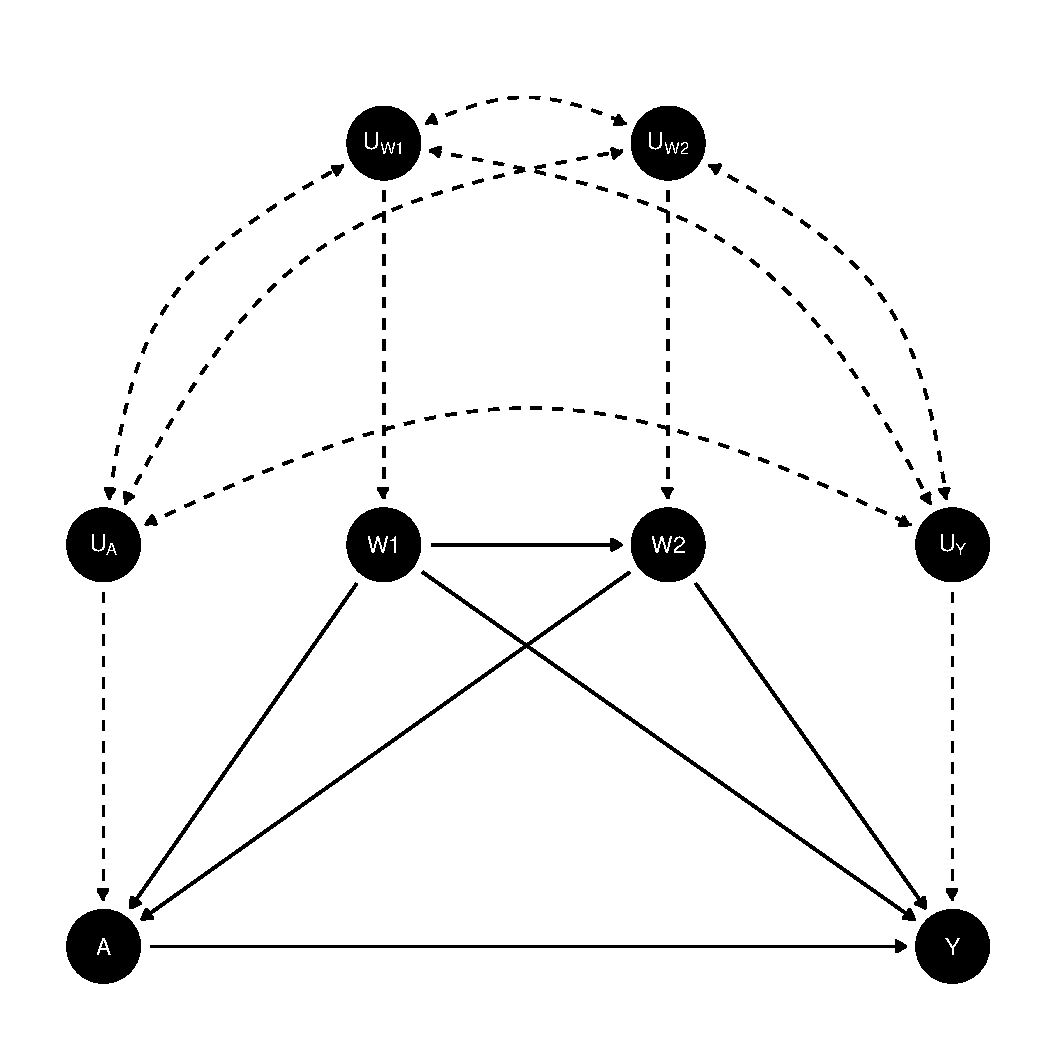
\includegraphics[width=4in]{figure/unnamed-chunk-16-1} 

\end{knitrout}
      
      
      
\end{document}
